%%%%%%%%%%%%%%%%%%%%%%%%%%%%%%%%%%%
\section{Métricas}
%%%%%%%%%%%%%%%%%%%%%%%%%%%%%%%%%%%
Nesta seção apresentamos métricas que tipicamente são utilizadas em análises de redes complexas. As métricas são 
baseadas na topologia da rede e podem ser usadas para identificar suas características.
% A seguir descrevemos 
% as principais métricas utilizadas no presente trabalho.

%%%%%%%%%%%%%%%%%%%%%%%%%%%%%%%%%%%
\subsection{Grau dos Nodos}
%%%%%%%%%%%%%%%%%%%%%%%%%%%%%%%%%%%

O grau de um nodo é o número de arestas incidentes àquele nodo, com os laços (uma aresta que possui o mesmo nodo 
como origem e destino) contando duas vezes. Esta é uma característica importante na estrutura da rede e segue a lei de 
potência em vários tipos de rede, como a Internet~\citep{Faloutsos1999}, a Web~\citep{Barabasi1999} e redes 
neurais~\citep{Braitenberg1998}. Sendo assim, a probabilidade de um nodo ter grau $k$ é proporcional a $k^{-\alpha}$, 
sendo $\alpha$ uma constante obtida através de regressão linear. Este expoente é comumente utilizado para comparar diferentes 
redes e seus valores variam entre 1,0 e 3,5 \citep{Ebel2002}. Em grafos direcionados, é comum analisar o grau dos nodos 
levando em consideração as arestas de entrada e de saída. Por exemplo, em uma rede de coautoria, um pesquisador é 
representado por um nodo, cujo grau indica o seu número de coautores.


%%%%%%%%%%%%%%%%%%%%%%%%%%%%%%%%%%%
\subsection{Coeficiente de Agrupamento}
%%%%%%%%%%%%%%%%%%%%%%%%%%%%%%%%%%%

O coeficiente de agrupamento (\textit{clustering coefficient}) é um indicador de conectividade entre os nodos de um 
grafo. Este indicador informa o quão agrupados os vizinhos de um dado nodo se encontram na rede, i.e., o coeficiente de 
agrupamento indica o quão interligados estão os coautores de um dado pesquisador na rede. Isto acontece porque os 
nodos tendem a criar grupos coesos caracterizados por um denso número de ligações. Sendo assim, a probabilidade
de nodos se interconectarem na forma de grupos tende a ser maior do que ligações aleatórias na rede.

\cite{Figueiredo2011} define o coeficiente de agrupamento de um nodo $i$, que pertence ao conjunto de nodos $i \in N$ 
de um dado grafo, como sendo a fração de arestas que os vizinhos de $i$ possuem entre si e o máximo de arestas possíveis 
que poderiam existir entre eles. Sendo $d_i$ o grau do nodo $i$, o número máximo de arestas entre seus vizinhos é 
$\binom{d_i}{2}$, ou seja, quando todos os pares de vizinhos de $i$ estão interconectados. Assim, sendo $E_i$ o número de arestas 
entre os vizinhos de $i$, temos que o coeficiente de agrupamento $c_i$ do nodo $i$ é dado por:

\begin{equation}
\label{eq:coeficiente_agrupamento_nodo}
c_i = \frac{E_i}{\binom{d_i}{2}} = \frac{2E_i}{d_i(d_i-1)} .
\end{equation}

Note que o coeficiente de agrupamento definido na Equação~\ref{eq:coeficiente_agrupamento_nodo} é aplicável somente a nodos 
com grau maior que um. De acordo com \cite{Figueiredo2011}, utilizando o coeficiente de agrupamento de cada nodo, podemos 
obter o coeficiente de agrupamento de toda a rede calculando a respectiva média aritmética, conforme:

\begin{equation}
\label{eq:coeficiente_agrupamento_rede}
\textit{\=c} = \frac{1}{n}\sum_{i \in N}{c_i} .
\end{equation}

É importante ressaltar que a Equação~\ref{eq:coeficiente_agrupamento_rede} necessita que todos os nodos pertencentes a $N$ 
tenham seus coeficientes de agrupamento previamente calculados. Considerando a Figura~\ref{fig:coeficiente_agrupamento_antes}, onde cada nodo representa um pesquisador em uma rede de coautoria,
o pesquisador \textit{E} possui um coeficiente de agrupamento $1/3$, porque existe somente uma única aresta entre \textit{D-F}, sendo que temos três pares de pesquisadores 
\textit{D-F}, \textit{D-C}, e \textit{C-F}. Na Figura~\ref{fig:coeficiente_agrupamento_depois} podemos observar que o valor do coeficiente de agrupamento 
do pesquisador \textit{E} é incrementado para 1, porque existem três arestas entre \textit{D-F}, \textit{D-C}, e \textit{C-F} entre os 
mesmos três pares.

\begin{figure}[!htb]
  \begin{center}
    \subfloat[Antes de novas arestas se formarem]{%
    \label{fig:coeficiente_agrupamento_antes}
      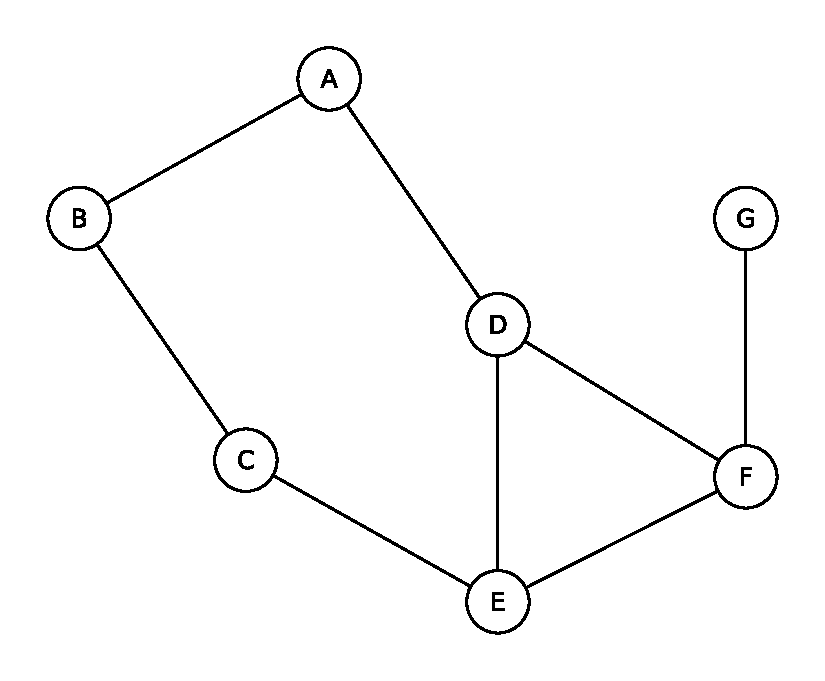
\includegraphics[scale=.55]{../imgs/coeficiente_agrupamento_1.eps}
    }%
    \subfloat[Depois de novas arestas se formarem]{%
      \label{fig:coeficiente_agrupamento_depois}
      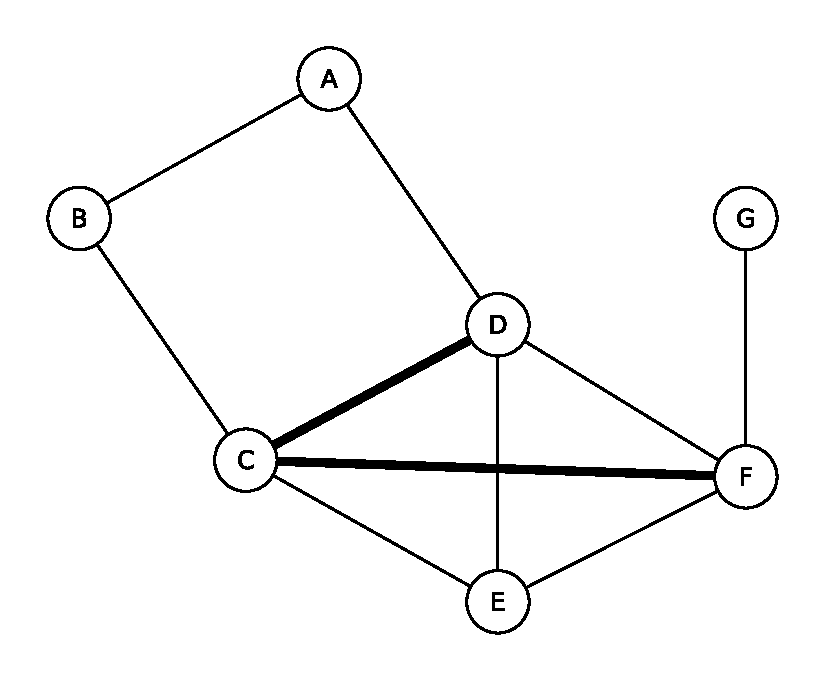
\includegraphics[scale=.55]{../imgs/coeficiente_agrupamento_2.eps}
    }%
  \end{center}
\caption{Exemplo de coeficiente de agrupamento}
\label{fig:averange_values_resemblance}
\end{figure}


%%%%%%%%%%%%%%%%%%%%%%%%%%%%%%%%%%%
\subsection{Componentes}
%%%%%%%%%%%%%%%%%%%%%%%%%%%%%%%%%%%

Segundo \cite{Easley2010}, um grafo é conectado quando existem arestas interligando todos os seus nodos. Naturalmente, 
um grafo é desconectado quando nem todos os seus nodos estão interligados, de modo que eles se dividem em grupos de nodos 
interconectados entre si, porém desconectados do restante da rede, sendo que dois grupos não se sobrepõem. Na 
Figura~\ref{fig:componentes_conectados}, podemos considerar que o grafo consiste de três partes, ou seja, três componentes
conectados: um composto pelos nodos \textit{K}, \textit{I}, \textit{J} e \textit{H}, outro composto pelos nodos 
\textit{L} e \textit{M} e o terceiro composto pelos demais nodos. Por exemplo, em uma rede de coautoria, poderíamos dizer
que cada componente é um grupo de pesquisa, sendo que os pesquisadores de um dado grupo não trabalham com pesquisadores
de outro grupo.

\cite{Easley2010} definem um componente conectado (\textit{connected component}), formalmente, como um subconjunto de 
nodos, tal que: (i) exista um caminho interligando todos os nodos daquele subconjunto e (ii) o subconjunto não é parte 
de um conjunto maior, onde cada nodo possa chegar a qualquer outro. Assim, podemos intuitivamente
definir que um componente é: (i) internamente conectado e (ii) como um todo, é uma ``parte'' 
desconectada das demais partes do grafo. Por exemplo, o subconjunto \textit{C}, \textit{F} e \textit{E} da 
Figura~\ref{fig:componentes_conectados} não poderia ser chamado de componente conectado, pois violaria a 
condição (ii). Embora o subconjunto atenda a condição (i), ele faz parte de um subconjunto maior que engloba 
o nodos de \textit{A} a \textit{G}.

\begin{figure}[!htb]
\centering
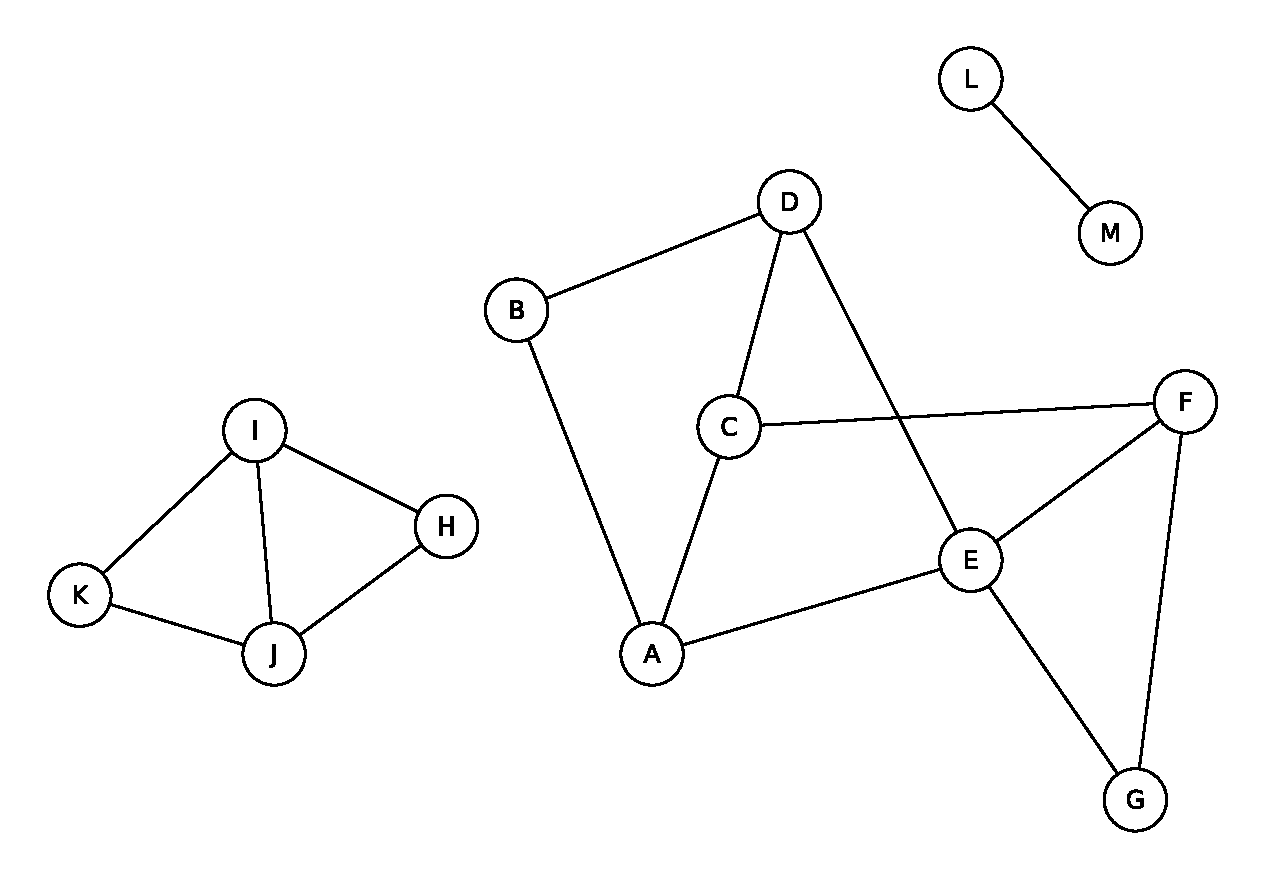
\includegraphics[scale=0.55]{../imgs/componentes.eps}
\caption{Um grafo com três componentes conectados}
\label{fig:componentes_conectados}
\end{figure}

Em um grafo direcionado, um componente é chamado de fortemente conectado quando existe pelo menos um caminho 
direcionado interligando todos os pares de nodos. Quando tal caminho existe, porém não direcionado, o componente 
é chamado de fracamente conectado. \cite{Benevenuto2012} exemplificam o modelo \textit{bow tie}, definido 
por \cite{Broder2000}, em que um grafo possui um componente central fortemente conectado, 
também chamado de \textit{core}, que pode ser alcançado ou alcançar outros grupos de componentes.

%%%%%%%%%%%%%%%%%%%%%%%%%%%%%%%%%%%
% \subsubsection{Maior Componente Conectado?}
%%%%%%%%%%%%%%%%%%%%%%%%%%%%%%%%%%%


%%%%%%%%%%%%%%%%%%%%%%%%%%%%%%%%%%%
\subsection{Caminho Mínimo Médio e Diâmetro}
%%%%%%%%%%%%%%%%%%%%%%%%%%%%%%%%%%%

Os caminhos de uma rede são um aspecto importante dela. Um caminho pode ser definido como uma sequência de nodos sem repetição
onde existe uma aresta entre cada par de nodos adjacentes na sequência. Por exemplo, na Figura~\ref{fig:componentes_conectados}
podemos dizer que existe um caminho entre \textit{A} e \textit{F}, sendo este caminho formado pelas arestas \textit{A-E} e 
\textit{E-F}. O comprimento de um caminho é dado pelo número de arestas que o define ou pelo número de nodos contidos no caminho
menos um. Ainda na Figura~\ref{fig:componentes_conectados}, o caminho contendo os nodos \textit{A}, \textit{B}, \textit{D}, \textit{C} e \textit{F} possui 
tamanho quatro.

Naturalmente existem muitos caminhos entre dois nodos quaisquer de um componente. Desta forma, o caminho mínimo entre
dois nodos é definido como sendo o comprimento do menor caminho entre eles. Assim, considerando os nodos  
\textit{A} e \textit{F} na Figura~\ref{fig:componentes_conectados}, o caminho mínimo entre eles é dois, definida pelos caminhos 
\textit{A}, \textit{C} e \textit{F} ou \textit{A}, \textit{E} e \textit{F}. 

O caminho mínimo médio de um grafo é a média do número de arestas em todos os caminhos mínimos existentes entre todos os pares 
de nodos do grafo. Geralmente esta medida é calculada no maior componente fortemente conectado para grafos direcionados ou no maior 
componente fracamente conectado para grafos não direcionados, uma vez que o grafo pode não ser totalmente conectado. \cite{Figueiredo2011} define 
o caminho mínimo médio como a média aritmética dos caminhos mínimos entre todos os pares de nodos da rede, sendo $l(i,j)$ o caminho mínimo entre os nodos
$i,j \in N$, onde $N$ é o conjuntos de nodos da rede. O caminho mínimo médio $\textit{\=l}$ é definido como:

\begin{equation}
\label{eq:distancia_media}
\textit{\=l} = \frac{\sum_{i,j \in N}{l(i,j)}}{\binom{n}{2}}.
\end{equation}

A Equação~\ref{eq:distancia_media} considera todos os pares não-ordenados, que ao todo são $\binom{n}{2}$. Outra métrica baseada 
em caminho mínimo é o diâmetro que também é calculado no maior componente fortemente conectado ou fracamente conectado. O 
diâmetro é o tamanho do maior caminho mínimo existente em todo o grafo, que \cite{Figueiredo2011} define como:

\begin{equation}
\label{eq:diametro}
\textit{L} = \max_{i,j\in N} l(i,j).
\end{equation}


%%%%%%%%%%%%%%%%%%%%%%%%%%%%%%%%%%%
\subsection{\textit{Betweenness}}
%%%%%%%%%%%%%%%%%%%%%%%%%%%%%%%%%%%

\textit{Betweenness} é uma métrica de centralidade que mede a importância de um determinado nodo ou aresta na rede 
referente à sua localização, considerando o número de caminhos mínimos que por ali passam. Nodos ou arestas com maior 
valor de \textit{betweenness} fazem parte de um número maior de caminhos mínimos e por isto são mais importantes na rede.

O valor da métrica \textit{betweenness} $B(e)$ de uma aresta $e$ pode, de acordo com \cite{Benevenuto2012}, ser formalmente definido como o 
número de caminhos mínimos entre todos os pares de nodos que passam por $e$. Desta forma temos:

\begin{equation}
\label{eq:betweenness}
B(e)=\sum_{u \in N, v \in N} \frac{\sigma_e (u,v)}{\sigma (u,v)}
\end{equation}
onde $\sigma (u,v)$ representa o número de caminhos mínimos entre $u$ e $v$, e $\sigma_e (u,v)$ representa o número de 
caminhos mínimos que incluem $e$. Assim, se existem vários caminhos mínimos entre $u$ e $v$, cada caminho recebe
um peso de modo que o somatório dos pesos seja um.

De forma análoga, o valor da métrica \textit{betweenness} pode ser computado para um nodo da rede ao invés de uma aresta. Assim teríamos
essa métrica representando a importância de um dado nodo para a rede, onde os vários caminhos mínimos que passam
por ele representam, de forma quantitativa, sua importância na rede. Por exemplo, em uma rede de coautoria, a existência de nodos com um alto valor
para a métrica \textit{betweenness} pode indicar que os respectivos pesquisadores atuam como pontes interligando vários grupos de pesquisa na rede. 
Desta forma, adotamos esta métrica de centralidade no restante da dissertação.

%%%%%%%%%%%%%%%%%%%%%%%%%%%%%%%%%%%
\subsection{Assortatividade}
%%%%%%%%%%%%%%%%%%%%%%%%%%%%%%%%%%%

A assortividade (\textit{assortativity} ou \textit{assortative mixing}) é uma métrica clássica de redes complexas que identifica
o comportamento de como os nodos tendem a se agrupar na rede, e.g., uma rede de coautoria apresenta propriedades assortativas 
quando pesquisadores com o mesmo número de conexões tendem a se conectar com outros pesquisadores com o mesmo número de conexões.

A assortatividade pode ser representada visualmente a partir de um gráfico em que cada grau $k$ encontrado em pelo menos um
nodo da rede é representado pelo grau médio $k_{nn}$ dos vizinhos dos nodos de grau $k$. Em grafos direcionados, este gráfico pode
ser construído separadamente para graus de entrada e graus de saída. Segundo \cite{Ahn2007}, esta métrica também pode ser expressa 
numericamente utilizando o coeficiente de correlação de Pearson:

\begin{equation}
\label{eq:assortatividade}
r = \frac{\langle k_ik_j \rangle-\langle k_i \rangle \langle k_j \rangle }
         {\sqrt{(\langle k^2_i \rangle - \langle k_i \rangle^2)(\langle k^2_j \rangle - \langle k_j \rangle^2)}}
\end{equation}
onde $k_i$ e $k_j$ são os graus dos nodos que constituem uma aresta e a notação $\langle \rangle$ representa a média sobre 
todas as arestas da rede.

Se a rede possui assortatividade negativa, nodos que possuem grau elevado tendem a se conectar a nodos com menor grau,
e vice versa. O coeficiente $r$ pode variar entre -1 e 1, onde $r > 0$ indica que a rede possui propriedades assortativas,
ou seja, nodos com graus semelhantes tendem a estabelecer conexões na rede, já $r < 0$ indica que a rede possui
propriedades disassortativas, existindo maior probabilidade de encontrar arestas entre nodos de graus diferentes.
Por exemplo, uma rede de coautoria com assortatividade negativa pode indicar que os pesquisadores seniores estão se
conectando a pesquisadores menos experientes, e.g., alunos de doutorado.